% SOURCE: gate_readout.json fields cells.*.c3.{nf4dq,int8}.median_ratio_mean; cells.*.c3.{nf4dq,int8}.r_func_mean; cells.*.c3.{nf4dq,int8}.r_param_mean.
% !TEX encoding = UTF-8 Unicode
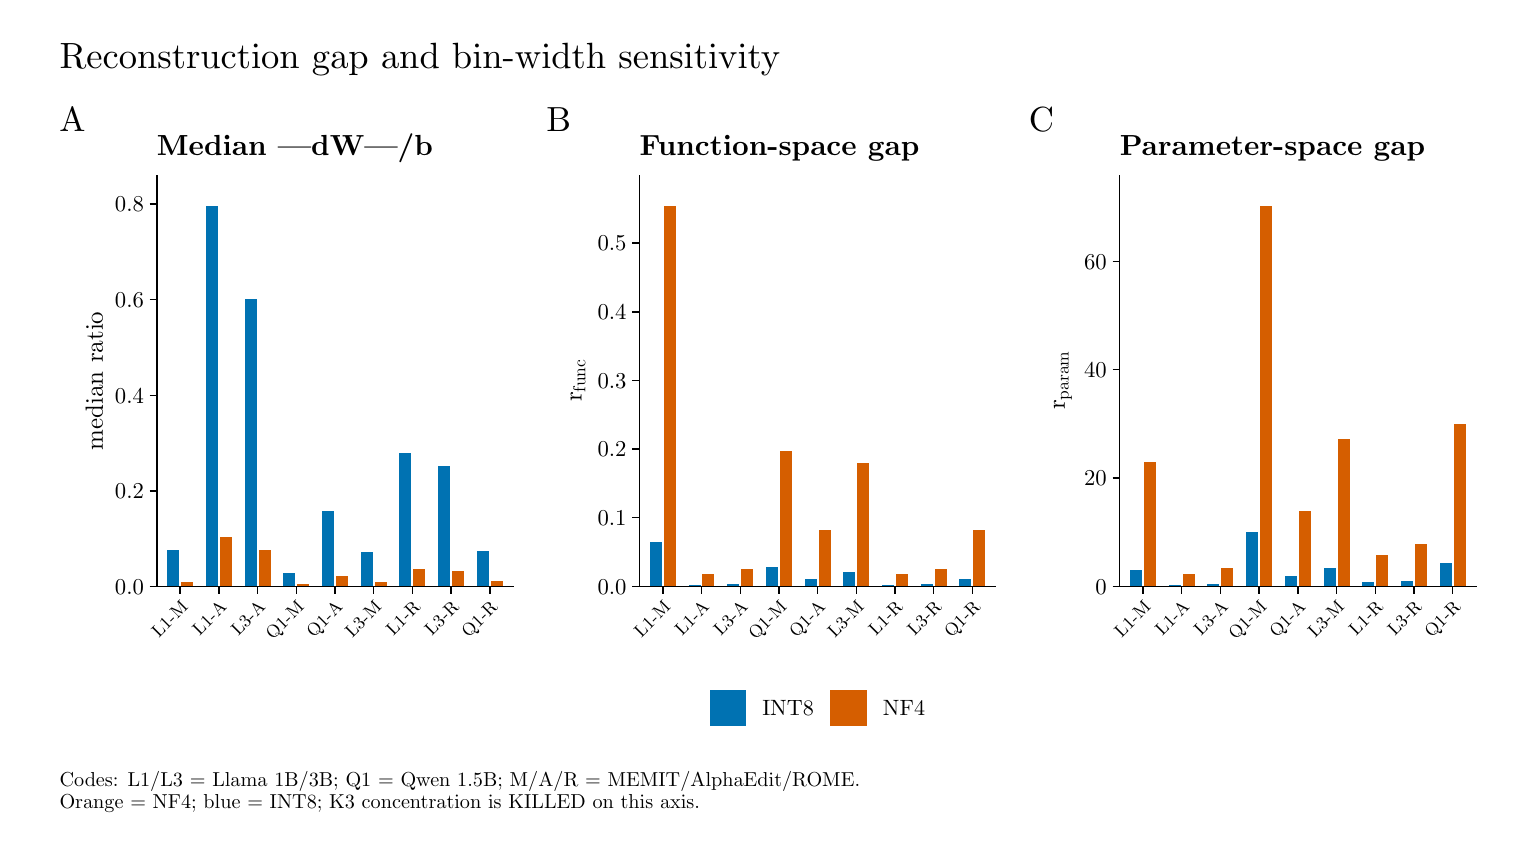
\begin{tikzpicture}[x=1pt,y=1pt]
\definecolor{fillColor}{RGB}{255,255,255}
\path[use as bounding box,fill=fillColor,fill opacity=0.00] (0,0) rectangle (534.80,289.08);
\begin{scope}
\path[clip] (  0.00,  0.00) rectangle (534.80,289.08);
\definecolor{drawColor}{RGB}{255,255,255}
\definecolor{fillColor}{RGB}{255,255,255}

\path[draw=drawColor,line width= 0.6pt,line join=round,line cap=round,fill=fillColor] ( -0.00,  0.00) rectangle (534.80,289.08);
\end{scope}
\begin{scope}
\path[clip] (  5.50, 24.83) rectangle (181.39,266.42);
\definecolor{drawColor}{RGB}{255,255,255}
\definecolor{fillColor}{RGB}{255,255,255}

\path[draw=drawColor,line width= 0.5pt,line join=round,line cap=round,fill=fillColor] (  5.50, 24.83) rectangle (181.39,266.42);
\end{scope}
\begin{scope}
\path[clip] (181.39, 24.83) rectangle (355.78,266.42);
\definecolor{drawColor}{RGB}{255,255,255}
\definecolor{fillColor}{RGB}{255,255,255}

\path[draw=drawColor,line width= 0.5pt,line join=round,line cap=round,fill=fillColor] (181.39, 24.83) rectangle (355.78,266.42);
\end{scope}
\begin{scope}
\path[clip] (355.78, 24.83) rectangle (529.30,266.42);
\definecolor{drawColor}{RGB}{255,255,255}
\definecolor{fillColor}{RGB}{255,255,255}

\path[draw=drawColor,line width= 0.5pt,line join=round,line cap=round,fill=fillColor] (355.78, 24.83) rectangle (529.30,266.42);
\end{scope}
\begin{scope}
\path[clip] ( 46.72, 87.18) rectangle (175.39,235.76);
\definecolor{fillColor}{RGB}{255,255,255}

\path[fill=fillColor] ( 46.72, 87.18) rectangle (175.39,235.76);
\definecolor{fillColor}{RGB}{213,94,0}

\path[fill=fillColor] ( 55.46, 87.18) rectangle ( 59.80, 88.85);
\definecolor{fillColor}{RGB}{0,114,178}

\path[fill=fillColor] ( 50.43, 87.18) rectangle ( 54.76,100.24);
\definecolor{fillColor}{RGB}{213,94,0}

\path[fill=fillColor] ( 69.45, 87.18) rectangle ( 73.78,105.11);
\definecolor{fillColor}{RGB}{0,114,178}

\path[fill=fillColor] ( 64.41, 87.18) rectangle ( 68.75,224.75);
\definecolor{fillColor}{RGB}{213,94,0}

\path[fill=fillColor] ( 83.43, 87.18) rectangle ( 87.77,100.30);
\definecolor{fillColor}{RGB}{0,114,178}

\path[fill=fillColor] ( 78.40, 87.18) rectangle ( 82.73,191.10);
\definecolor{fillColor}{RGB}{213,94,0}

\path[fill=fillColor] ( 97.42, 87.18) rectangle (101.75, 87.90);
\definecolor{fillColor}{RGB}{0,114,178}

\path[fill=fillColor] ( 92.38, 87.18) rectangle ( 96.72, 92.17);
\definecolor{fillColor}{RGB}{213,94,0}

\path[fill=fillColor] (111.40, 87.18) rectangle (115.74, 91.07);
\definecolor{fillColor}{RGB}{0,114,178}

\path[fill=fillColor] (106.37, 87.18) rectangle (110.70,114.57);
\definecolor{fillColor}{RGB}{213,94,0}

\path[fill=fillColor] (125.39, 87.18) rectangle (129.72, 88.74);
\definecolor{fillColor}{RGB}{0,114,178}

\path[fill=fillColor] (120.35, 87.18) rectangle (124.69, 99.56);
\definecolor{fillColor}{RGB}{213,94,0}

\path[fill=fillColor] (139.37, 87.18) rectangle (143.71, 93.38);
\definecolor{fillColor}{RGB}{0,114,178}

\path[fill=fillColor] (134.34, 87.18) rectangle (138.68,135.56);
\definecolor{fillColor}{RGB}{213,94,0}

\path[fill=fillColor] (153.36, 87.18) rectangle (157.70, 92.62);
\definecolor{fillColor}{RGB}{0,114,178}

\path[fill=fillColor] (148.33, 87.18) rectangle (152.66,130.52);
\definecolor{fillColor}{RGB}{213,94,0}

\path[fill=fillColor] (167.35, 87.18) rectangle (171.68, 88.98);
\definecolor{fillColor}{RGB}{0,114,178}

\path[fill=fillColor] (162.31, 87.18) rectangle (166.65, 99.85);
\end{scope}
\begin{scope}
\path[clip] (  0.00,  0.00) rectangle (534.80,289.08);
\definecolor{drawColor}{RGB}{0,0,0}

\path[draw=drawColor,line width= 0.5pt,line join=round,line cap=rect] ( 46.72, 87.18) --
	( 46.72,235.76);
\end{scope}
\begin{scope}
\path[clip] (  0.00,  0.00) rectangle (534.80,289.08);
\definecolor{drawColor}{RGB}{0,0,0}

\node[text=drawColor,anchor=base east,inner sep=0pt, outer sep=0pt, scale=  0.82] at ( 42.00, 84.36) {0.0};

\node[text=drawColor,anchor=base east,inner sep=0pt, outer sep=0pt, scale=  0.82] at ( 42.00,118.89) {0.2};

\node[text=drawColor,anchor=base east,inner sep=0pt, outer sep=0pt, scale=  0.82] at ( 42.00,153.43) {0.4};

\node[text=drawColor,anchor=base east,inner sep=0pt, outer sep=0pt, scale=  0.82] at ( 42.00,187.96) {0.6};

\node[text=drawColor,anchor=base east,inner sep=0pt, outer sep=0pt, scale=  0.82] at ( 42.00,222.50) {0.8};
\end{scope}
\begin{scope}
\path[clip] (  0.00,  0.00) rectangle (534.80,289.08);
\definecolor{drawColor}{RGB}{0,0,0}

\path[draw=drawColor,line width= 0.5pt,line join=round] ( 44.10, 87.18) --
	( 46.72, 87.18);

\path[draw=drawColor,line width= 0.5pt,line join=round] ( 44.10,121.72) --
	( 46.72,121.72);

\path[draw=drawColor,line width= 0.5pt,line join=round] ( 44.10,156.25) --
	( 46.72,156.25);

\path[draw=drawColor,line width= 0.5pt,line join=round] ( 44.10,190.79) --
	( 46.72,190.79);

\path[draw=drawColor,line width= 0.5pt,line join=round] ( 44.10,225.32) --
	( 46.72,225.32);
\end{scope}
\begin{scope}
\path[clip] (  0.00,  0.00) rectangle (534.80,289.08);
\definecolor{drawColor}{RGB}{0,0,0}

\path[draw=drawColor,line width= 0.5pt,line join=round,line cap=rect] ( 46.72, 87.18) --
	(175.39, 87.18);
\end{scope}
\begin{scope}
\path[clip] (  0.00,  0.00) rectangle (534.80,289.08);
\definecolor{drawColor}{RGB}{0,0,0}

\path[draw=drawColor,line width= 0.5pt,line join=round] ( 55.11, 84.56) --
	( 55.11, 87.18);

\path[draw=drawColor,line width= 0.5pt,line join=round] ( 69.10, 84.56) --
	( 69.10, 87.18);

\path[draw=drawColor,line width= 0.5pt,line join=round] ( 83.08, 84.56) --
	( 83.08, 87.18);

\path[draw=drawColor,line width= 0.5pt,line join=round] ( 97.07, 84.56) --
	( 97.07, 87.18);

\path[draw=drawColor,line width= 0.5pt,line join=round] (111.05, 84.56) --
	(111.05, 87.18);

\path[draw=drawColor,line width= 0.5pt,line join=round] (125.04, 84.56) --
	(125.04, 87.18);

\path[draw=drawColor,line width= 0.5pt,line join=round] (139.03, 84.56) --
	(139.03, 87.18);

\path[draw=drawColor,line width= 0.5pt,line join=round] (153.01, 84.56) --
	(153.01, 87.18);

\path[draw=drawColor,line width= 0.5pt,line join=round] (167.00, 84.56) --
	(167.00, 87.18);
\end{scope}
\begin{scope}
\path[clip] (  0.00,  0.00) rectangle (534.80,289.08);
\definecolor{drawColor}{RGB}{0,0,0}

\node[text=drawColor,rotate= 45.00,anchor=base east,inner sep=0pt, outer sep=0pt, scale=  0.65] at ( 58.28, 79.29) {L1-M};

\node[text=drawColor,rotate= 45.00,anchor=base east,inner sep=0pt, outer sep=0pt, scale=  0.65] at ( 72.26, 79.29) {L1-A};

\node[text=drawColor,rotate= 45.00,anchor=base east,inner sep=0pt, outer sep=0pt, scale=  0.65] at ( 86.25, 79.29) {L3-A};

\node[text=drawColor,rotate= 45.00,anchor=base east,inner sep=0pt, outer sep=0pt, scale=  0.65] at (100.23, 79.29) {Q1-M};

\node[text=drawColor,rotate= 45.00,anchor=base east,inner sep=0pt, outer sep=0pt, scale=  0.65] at (114.22, 79.29) {Q1-A};

\node[text=drawColor,rotate= 45.00,anchor=base east,inner sep=0pt, outer sep=0pt, scale=  0.65] at (128.21, 79.29) {L3-M};

\node[text=drawColor,rotate= 45.00,anchor=base east,inner sep=0pt, outer sep=0pt, scale=  0.65] at (142.19, 79.29) {L1-R};

\node[text=drawColor,rotate= 45.00,anchor=base east,inner sep=0pt, outer sep=0pt, scale=  0.65] at (156.18, 79.29) {L3-R};

\node[text=drawColor,rotate= 45.00,anchor=base east,inner sep=0pt, outer sep=0pt, scale=  0.65] at (170.16, 79.29) {Q1-R};
\end{scope}
\begin{scope}
\path[clip] (  0.00,  0.00) rectangle (534.80,289.08);
\definecolor{drawColor}{RGB}{0,0,0}

\node[text=drawColor,rotate= 90.00,anchor=base,inner sep=0pt, outer sep=0pt, scale=  0.90] at ( 27.15,161.47) {median ratio};
\end{scope}
\begin{scope}
\path[clip] (  0.00,  0.00) rectangle (534.80,289.08);
\definecolor{drawColor}{RGB}{0,0,0}

\node[text=drawColor,anchor=base west,inner sep=0pt, outer sep=0pt, scale=  1.05] at ( 46.72,243.05) {\bfseries Median |dW|/b};
\end{scope}
\begin{scope}
\path[clip] (  0.00,  0.00) rectangle (534.80,289.08);
\definecolor{drawColor}{RGB}{0,0,0}

\node[text=drawColor,anchor=base,inner sep=0pt, outer sep=0pt, scale=  1.26] at ( 16.22,251.52) {A};
\end{scope}
\begin{scope}
\path[clip] (221.12, 87.18) rectangle (349.78,235.76);
\definecolor{fillColor}{RGB}{255,255,255}

\path[fill=fillColor] (221.12, 87.18) rectangle (349.78,235.76);
\definecolor{fillColor}{RGB}{213,94,0}

\path[fill=fillColor] (229.86, 87.18) rectangle (234.19,224.75);
\definecolor{fillColor}{RGB}{0,114,178}

\path[fill=fillColor] (224.82, 87.18) rectangle (229.16,103.37);
\definecolor{fillColor}{RGB}{213,94,0}

\path[fill=fillColor] (243.84, 87.18) rectangle (248.18, 91.67);
\definecolor{fillColor}{RGB}{0,114,178}

\path[fill=fillColor] (238.81, 87.18) rectangle (243.14, 87.68);
\definecolor{fillColor}{RGB}{213,94,0}

\path[fill=fillColor] (257.83, 87.18) rectangle (262.16, 93.53);
\definecolor{fillColor}{RGB}{0,114,178}

\path[fill=fillColor] (252.79, 87.18) rectangle (257.13, 87.87);
\definecolor{fillColor}{RGB}{213,94,0}

\path[fill=fillColor] (271.81, 87.18) rectangle (276.15,136.17);
\definecolor{fillColor}{RGB}{0,114,178}

\path[fill=fillColor] (266.78, 87.18) rectangle (271.11, 94.12);
\definecolor{fillColor}{RGB}{213,94,0}

\path[fill=fillColor] (285.80, 87.18) rectangle (290.13,107.51);
\definecolor{fillColor}{RGB}{0,114,178}

\path[fill=fillColor] (280.76, 87.18) rectangle (285.10, 89.98);
\definecolor{fillColor}{RGB}{213,94,0}

\path[fill=fillColor] (299.78, 87.18) rectangle (304.12,131.88);
\definecolor{fillColor}{RGB}{0,114,178}

\path[fill=fillColor] (294.75, 87.18) rectangle (299.08, 92.25);
\definecolor{fillColor}{RGB}{213,94,0}

\path[fill=fillColor] (313.77, 87.18) rectangle (318.10, 91.76);
\definecolor{fillColor}{RGB}{0,114,178}

\path[fill=fillColor] (308.73, 87.18) rectangle (313.07, 87.67);
\definecolor{fillColor}{RGB}{213,94,0}

\path[fill=fillColor] (327.75, 87.18) rectangle (332.09, 93.61);
\definecolor{fillColor}{RGB}{0,114,178}

\path[fill=fillColor] (322.72, 87.18) rectangle (327.06, 87.87);
\definecolor{fillColor}{RGB}{213,94,0}

\path[fill=fillColor] (341.74, 87.18) rectangle (346.08,107.45);
\definecolor{fillColor}{RGB}{0,114,178}

\path[fill=fillColor] (336.71, 87.18) rectangle (341.04, 90.02);
\end{scope}
\begin{scope}
\path[clip] (  0.00,  0.00) rectangle (534.80,289.08);
\definecolor{drawColor}{RGB}{0,0,0}

\path[draw=drawColor,line width= 0.5pt,line join=round,line cap=rect] (221.12, 87.18) --
	(221.12,235.76);
\end{scope}
\begin{scope}
\path[clip] (  0.00,  0.00) rectangle (534.80,289.08);
\definecolor{drawColor}{RGB}{0,0,0}

\node[text=drawColor,anchor=base east,inner sep=0pt, outer sep=0pt, scale=  0.82] at (216.39, 84.36) {0.0};

\node[text=drawColor,anchor=base east,inner sep=0pt, outer sep=0pt, scale=  0.82] at (216.39,109.17) {0.1};

\node[text=drawColor,anchor=base east,inner sep=0pt, outer sep=0pt, scale=  0.82] at (216.39,133.97) {0.2};

\node[text=drawColor,anchor=base east,inner sep=0pt, outer sep=0pt, scale=  0.82] at (216.39,158.78) {0.3};

\node[text=drawColor,anchor=base east,inner sep=0pt, outer sep=0pt, scale=  0.82] at (216.39,183.58) {0.4};

\node[text=drawColor,anchor=base east,inner sep=0pt, outer sep=0pt, scale=  0.82] at (216.39,208.39) {0.5};
\end{scope}
\begin{scope}
\path[clip] (  0.00,  0.00) rectangle (534.80,289.08);
\definecolor{drawColor}{RGB}{0,0,0}

\path[draw=drawColor,line width= 0.5pt,line join=round] (218.49, 87.18) --
	(221.12, 87.18);

\path[draw=drawColor,line width= 0.5pt,line join=round] (218.49,111.99) --
	(221.12,111.99);

\path[draw=drawColor,line width= 0.5pt,line join=round] (218.49,136.79) --
	(221.12,136.79);

\path[draw=drawColor,line width= 0.5pt,line join=round] (218.49,161.60) --
	(221.12,161.60);

\path[draw=drawColor,line width= 0.5pt,line join=round] (218.49,186.40) --
	(221.12,186.40);

\path[draw=drawColor,line width= 0.5pt,line join=round] (218.49,211.21) --
	(221.12,211.21);
\end{scope}
\begin{scope}
\path[clip] (  0.00,  0.00) rectangle (534.80,289.08);
\definecolor{drawColor}{RGB}{0,0,0}

\path[draw=drawColor,line width= 0.5pt,line join=round,line cap=rect] (221.12, 87.18) --
	(349.78, 87.18);
\end{scope}
\begin{scope}
\path[clip] (  0.00,  0.00) rectangle (534.80,289.08);
\definecolor{drawColor}{RGB}{0,0,0}

\path[draw=drawColor,line width= 0.5pt,line join=round] (229.51, 84.56) --
	(229.51, 87.18);

\path[draw=drawColor,line width= 0.5pt,line join=round] (243.49, 84.56) --
	(243.49, 87.18);

\path[draw=drawColor,line width= 0.5pt,line join=round] (257.48, 84.56) --
	(257.48, 87.18);

\path[draw=drawColor,line width= 0.5pt,line join=round] (271.46, 84.56) --
	(271.46, 87.18);

\path[draw=drawColor,line width= 0.5pt,line join=round] (285.45, 84.56) --
	(285.45, 87.18);

\path[draw=drawColor,line width= 0.5pt,line join=round] (299.43, 84.56) --
	(299.43, 87.18);

\path[draw=drawColor,line width= 0.5pt,line join=round] (313.42, 84.56) --
	(313.42, 87.18);

\path[draw=drawColor,line width= 0.5pt,line join=round] (327.40, 84.56) --
	(327.40, 87.18);

\path[draw=drawColor,line width= 0.5pt,line join=round] (341.39, 84.56) --
	(341.39, 87.18);
\end{scope}
\begin{scope}
\path[clip] (  0.00,  0.00) rectangle (534.80,289.08);
\definecolor{drawColor}{RGB}{0,0,0}

\node[text=drawColor,rotate= 45.00,anchor=base east,inner sep=0pt, outer sep=0pt, scale=  0.65] at (232.67, 79.29) {L1-M};

\node[text=drawColor,rotate= 45.00,anchor=base east,inner sep=0pt, outer sep=0pt, scale=  0.65] at (246.66, 79.29) {L1-A};

\node[text=drawColor,rotate= 45.00,anchor=base east,inner sep=0pt, outer sep=0pt, scale=  0.65] at (260.64, 79.29) {L3-A};

\node[text=drawColor,rotate= 45.00,anchor=base east,inner sep=0pt, outer sep=0pt, scale=  0.65] at (274.63, 79.29) {Q1-M};

\node[text=drawColor,rotate= 45.00,anchor=base east,inner sep=0pt, outer sep=0pt, scale=  0.65] at (288.61, 79.29) {Q1-A};

\node[text=drawColor,rotate= 45.00,anchor=base east,inner sep=0pt, outer sep=0pt, scale=  0.65] at (302.60, 79.29) {L3-M};

\node[text=drawColor,rotate= 45.00,anchor=base east,inner sep=0pt, outer sep=0pt, scale=  0.65] at (316.58, 79.29) {L1-R};

\node[text=drawColor,rotate= 45.00,anchor=base east,inner sep=0pt, outer sep=0pt, scale=  0.65] at (330.57, 79.29) {L3-R};

\node[text=drawColor,rotate= 45.00,anchor=base east,inner sep=0pt, outer sep=0pt, scale=  0.65] at (344.56, 79.29) {Q1-R};
\end{scope}
\begin{scope}
\path[clip] (  0.00,  0.00) rectangle (534.80,289.08);
\definecolor{drawColor}{RGB}{0,0,0}

\node[text=drawColor,rotate= 90.00,anchor=base west,inner sep=0pt, outer sep=0pt, scale=  0.90] at (200.18,153.85) {r};

\node[text=drawColor,rotate= 90.00,anchor=base west,inner sep=0pt, outer sep=0pt, scale=  0.63] at (201.54,157.37) {f};

\node[text=drawColor,rotate= 90.00,anchor=base west,inner sep=0pt, outer sep=0pt, scale=  0.63] at (201.54,159.30) {u};

\node[text=drawColor,rotate= 90.00,anchor=base west,inner sep=0pt, outer sep=0pt, scale=  0.63] at (201.54,162.80) {n};

\node[text=drawColor,rotate= 90.00,anchor=base west,inner sep=0pt, outer sep=0pt, scale=  0.63] at (201.54,166.29) {c};
\end{scope}
\begin{scope}
\path[clip] (  0.00,  0.00) rectangle (534.80,289.08);
\definecolor{drawColor}{RGB}{0,0,0}

\node[text=drawColor,anchor=base west,inner sep=0pt, outer sep=0pt, scale=  1.05] at (221.12,243.05) {\bfseries Function-space gap};
\end{scope}
\begin{scope}
\path[clip] (  0.00,  0.00) rectangle (534.80,289.08);
\definecolor{drawColor}{RGB}{0,0,0}

\node[text=drawColor,anchor=base,inner sep=0pt, outer sep=0pt, scale=  1.26] at (191.85,251.52) {B};
\end{scope}
\begin{scope}
\path[clip] (394.63, 87.18) rectangle (523.30,235.76);
\definecolor{fillColor}{RGB}{255,255,255}

\path[fill=fillColor] (394.63, 87.18) rectangle (523.30,235.76);
\definecolor{fillColor}{RGB}{213,94,0}

\path[fill=fillColor] (403.37, 87.18) rectangle (407.71,132.06);
\definecolor{fillColor}{RGB}{0,114,178}

\path[fill=fillColor] (398.34, 87.18) rectangle (402.67, 93.05);
\definecolor{fillColor}{RGB}{213,94,0}

\path[fill=fillColor] (417.36, 87.18) rectangle (421.69, 91.65);
\definecolor{fillColor}{RGB}{0,114,178}

\path[fill=fillColor] (412.32, 87.18) rectangle (416.66, 87.78);
\definecolor{fillColor}{RGB}{213,94,0}

\path[fill=fillColor] (431.34, 87.18) rectangle (435.68, 93.82);
\definecolor{fillColor}{RGB}{0,114,178}

\path[fill=fillColor] (426.31, 87.18) rectangle (430.64, 88.03);
\definecolor{fillColor}{RGB}{213,94,0}

\path[fill=fillColor] (445.33, 87.18) rectangle (449.66,224.75);
\definecolor{fillColor}{RGB}{0,114,178}

\path[fill=fillColor] (440.29, 87.18) rectangle (444.63,106.82);
\definecolor{fillColor}{RGB}{213,94,0}

\path[fill=fillColor] (459.31, 87.18) rectangle (463.65,114.30);
\definecolor{fillColor}{RGB}{0,114,178}

\path[fill=fillColor] (454.28, 87.18) rectangle (458.62, 91.05);
\definecolor{fillColor}{RGB}{213,94,0}

\path[fill=fillColor] (473.30, 87.18) rectangle (477.64,140.55);
\definecolor{fillColor}{RGB}{0,114,178}

\path[fill=fillColor] (468.27, 87.18) rectangle (472.60, 93.99);
\definecolor{fillColor}{RGB}{213,94,0}

\path[fill=fillColor] (487.29, 87.18) rectangle (491.62, 98.57);
\definecolor{fillColor}{RGB}{0,114,178}

\path[fill=fillColor] (482.25, 87.18) rectangle (486.59, 88.67);
\definecolor{fillColor}{RGB}{213,94,0}

\path[fill=fillColor] (501.27, 87.18) rectangle (505.61,102.42);
\definecolor{fillColor}{RGB}{0,114,178}

\path[fill=fillColor] (496.24, 87.18) rectangle (500.57, 89.12);
\definecolor{fillColor}{RGB}{213,94,0}

\path[fill=fillColor] (515.26, 87.18) rectangle (519.59,145.76);
\definecolor{fillColor}{RGB}{0,114,178}

\path[fill=fillColor] (510.22, 87.18) rectangle (514.56, 95.55);
\end{scope}
\begin{scope}
\path[clip] (  0.00,  0.00) rectangle (534.80,289.08);
\definecolor{drawColor}{RGB}{0,0,0}

\path[draw=drawColor,line width= 0.5pt,line join=round,line cap=rect] (394.63, 87.18) --
	(394.63,235.76);
\end{scope}
\begin{scope}
\path[clip] (  0.00,  0.00) rectangle (534.80,289.08);
\definecolor{drawColor}{RGB}{0,0,0}

\node[text=drawColor,anchor=base east,inner sep=0pt, outer sep=0pt, scale=  0.82] at (389.91, 84.36) {0};

\node[text=drawColor,anchor=base east,inner sep=0pt, outer sep=0pt, scale=  0.82] at (389.91,123.50) {20};

\node[text=drawColor,anchor=base east,inner sep=0pt, outer sep=0pt, scale=  0.82] at (389.91,162.63) {40};

\node[text=drawColor,anchor=base east,inner sep=0pt, outer sep=0pt, scale=  0.82] at (389.91,201.77) {60};
\end{scope}
\begin{scope}
\path[clip] (  0.00,  0.00) rectangle (534.80,289.08);
\definecolor{drawColor}{RGB}{0,0,0}

\path[draw=drawColor,line width= 0.5pt,line join=round] (392.01, 87.18) --
	(394.63, 87.18);

\path[draw=drawColor,line width= 0.5pt,line join=round] (392.01,126.32) --
	(394.63,126.32);

\path[draw=drawColor,line width= 0.5pt,line join=round] (392.01,165.46) --
	(394.63,165.46);

\path[draw=drawColor,line width= 0.5pt,line join=round] (392.01,204.59) --
	(394.63,204.59);
\end{scope}
\begin{scope}
\path[clip] (  0.00,  0.00) rectangle (534.80,289.08);
\definecolor{drawColor}{RGB}{0,0,0}

\path[draw=drawColor,line width= 0.5pt,line join=round,line cap=rect] (394.63, 87.18) --
	(523.30, 87.18);
\end{scope}
\begin{scope}
\path[clip] (  0.00,  0.00) rectangle (534.80,289.08);
\definecolor{drawColor}{RGB}{0,0,0}

\path[draw=drawColor,line width= 0.5pt,line join=round] (403.02, 84.56) --
	(403.02, 87.18);

\path[draw=drawColor,line width= 0.5pt,line join=round] (417.01, 84.56) --
	(417.01, 87.18);

\path[draw=drawColor,line width= 0.5pt,line join=round] (430.99, 84.56) --
	(430.99, 87.18);

\path[draw=drawColor,line width= 0.5pt,line join=round] (444.98, 84.56) --
	(444.98, 87.18);

\path[draw=drawColor,line width= 0.5pt,line join=round] (458.96, 84.56) --
	(458.96, 87.18);

\path[draw=drawColor,line width= 0.5pt,line join=round] (472.95, 84.56) --
	(472.95, 87.18);

\path[draw=drawColor,line width= 0.5pt,line join=round] (486.94, 84.56) --
	(486.94, 87.18);

\path[draw=drawColor,line width= 0.5pt,line join=round] (500.92, 84.56) --
	(500.92, 87.18);

\path[draw=drawColor,line width= 0.5pt,line join=round] (514.91, 84.56) --
	(514.91, 87.18);
\end{scope}
\begin{scope}
\path[clip] (  0.00,  0.00) rectangle (534.80,289.08);
\definecolor{drawColor}{RGB}{0,0,0}

\node[text=drawColor,rotate= 45.00,anchor=base east,inner sep=0pt, outer sep=0pt, scale=  0.65] at (406.19, 79.29) {L1-M};

\node[text=drawColor,rotate= 45.00,anchor=base east,inner sep=0pt, outer sep=0pt, scale=  0.65] at (420.17, 79.29) {L1-A};

\node[text=drawColor,rotate= 45.00,anchor=base east,inner sep=0pt, outer sep=0pt, scale=  0.65] at (434.16, 79.29) {L3-A};

\node[text=drawColor,rotate= 45.00,anchor=base east,inner sep=0pt, outer sep=0pt, scale=  0.65] at (448.14, 79.29) {Q1-M};

\node[text=drawColor,rotate= 45.00,anchor=base east,inner sep=0pt, outer sep=0pt, scale=  0.65] at (462.13, 79.29) {Q1-A};

\node[text=drawColor,rotate= 45.00,anchor=base east,inner sep=0pt, outer sep=0pt, scale=  0.65] at (476.12, 79.29) {L3-M};

\node[text=drawColor,rotate= 45.00,anchor=base east,inner sep=0pt, outer sep=0pt, scale=  0.65] at (490.10, 79.29) {L1-R};

\node[text=drawColor,rotate= 45.00,anchor=base east,inner sep=0pt, outer sep=0pt, scale=  0.65] at (504.09, 79.29) {L3-R};

\node[text=drawColor,rotate= 45.00,anchor=base east,inner sep=0pt, outer sep=0pt, scale=  0.65] at (518.07, 79.29) {Q1-R};
\end{scope}
\begin{scope}
\path[clip] (  0.00,  0.00) rectangle (534.80,289.08);
\definecolor{drawColor}{RGB}{0,0,0}

\node[text=drawColor,rotate= 90.00,anchor=base west,inner sep=0pt, outer sep=0pt, scale=  0.90] at (374.75,150.95) {r};

\node[text=drawColor,rotate= 90.00,anchor=base west,inner sep=0pt, outer sep=0pt, scale=  0.63] at (376.11,154.48) {p};

\node[text=drawColor,rotate= 90.00,anchor=base west,inner sep=0pt, outer sep=0pt, scale=  0.63] at (376.11,157.98) {a};

\node[text=drawColor,rotate= 90.00,anchor=base west,inner sep=0pt, outer sep=0pt, scale=  0.63] at (376.11,161.12) {r};

\node[text=drawColor,rotate= 90.00,anchor=base west,inner sep=0pt, outer sep=0pt, scale=  0.63] at (376.11,163.59) {a};

\node[text=drawColor,rotate= 90.00,anchor=base west,inner sep=0pt, outer sep=0pt, scale=  0.63] at (376.11,166.74) {m};
\end{scope}
\begin{scope}
\path[clip] (  0.00,  0.00) rectangle (534.80,289.08);
\definecolor{drawColor}{RGB}{0,0,0}

\node[text=drawColor,anchor=base west,inner sep=0pt, outer sep=0pt, scale=  1.05] at (394.63,243.05) {\bfseries Parameter-space gap};
\end{scope}
\begin{scope}
\path[clip] (  0.00,  0.00) rectangle (534.80,289.08);
\definecolor{drawColor}{RGB}{0,0,0}

\node[text=drawColor,anchor=base,inner sep=0pt, outer sep=0pt, scale=  1.26] at (366.33,251.52) {C};
\end{scope}
\begin{scope}
\path[clip] (  0.00,  0.00) rectangle (534.80,289.08);
\definecolor{fillColor}{RGB}{255,255,255}

\path[fill=fillColor] (240.49, 30.83) rectangle (329.53, 55.78);
\end{scope}
\begin{scope}
\path[clip] (  0.00,  0.00) rectangle (534.80,289.08);
\definecolor{fillColor}{RGB}{255,255,255}

\path[fill=fillColor] (245.74, 36.08) rectangle (260.19, 50.53);
\definecolor{fillColor}{RGB}{0,114,178}

\path[fill=fillColor] (246.42, 36.76) rectangle (259.52, 49.86);
\end{scope}
\begin{scope}
\path[clip] (  0.00,  0.00) rectangle (534.80,289.08);
\definecolor{fillColor}{RGB}{255,255,255}

\path[fill=fillColor] (289.36, 36.08) rectangle (303.81, 50.53);
\definecolor{fillColor}{RGB}{213,94,0}

\path[fill=fillColor] (290.04, 36.76) rectangle (303.13, 49.86);
\end{scope}
\begin{scope}
\path[clip] (  0.00,  0.00) rectangle (534.80,289.08);
\definecolor{drawColor}{RGB}{0,0,0}

\node[text=drawColor,anchor=base west,inner sep=0pt, outer sep=0pt, scale=  0.80] at (265.44, 40.55) {INT8};
\end{scope}
\begin{scope}
\path[clip] (  0.00,  0.00) rectangle (534.80,289.08);
\definecolor{drawColor}{RGB}{0,0,0}

\node[text=drawColor,anchor=base west,inner sep=0pt, outer sep=0pt, scale=  0.80] at (309.06, 40.55) {NF4};
\end{scope}
\begin{scope}
\path[clip] (  0.00,  0.00) rectangle (534.80,289.08);
\definecolor{drawColor}{RGB}{0,0,0}

\node[text=drawColor,anchor=base west,inner sep=0pt, outer sep=0pt, scale=  0.73] at ( 11.50, 14.80) {Codes: L1/L3 = Llama 1B/3B; Q1 = Qwen 1.5B; M/A/R = MEMIT/AlphaEdit/ROME.};

\node[text=drawColor,anchor=base west,inner sep=0pt, outer sep=0pt, scale=  0.73] at ( 11.50,  6.92) {Orange = NF4; blue = INT8; K3 concentration is KILLED on this axis.};
\end{scope}
\begin{scope}
\path[clip] (  0.00,  0.00) rectangle (534.80,289.08);
\definecolor{drawColor}{RGB}{0,0,0}

\node[text=drawColor,anchor=base west,inner sep=0pt, outer sep=0pt, scale=  1.32] at ( 11.50,274.49) {Reconstruction gap and bin-width sensitivity};
\end{scope}
\end{tikzpicture}
